%!TEX root = ../../../main.tex

\subsection{IXMAS dataset}
    The IXMAS dataset is a multi-view dataset built by Perception project \cite{weinland2006free}.
    It contains 12 action classes (check watch, cross arms, scratch head, sit down, get up, turn around, walk, wave, punch, kick, point and pick up) recorded simultaneously by 5 cameras (4 side view cameras and 1 top view camera).
    Each action is performed 3 times by 10 actors (5 males / 5 females).
    Some representative frames of action \textit{check watch} are shown in Fig.\ref{Fig:IXMAS1}.

    \begin{figure}[h]
        \centering
        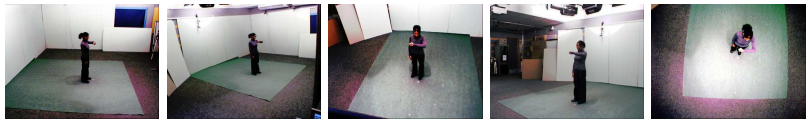
\includegraphics[width=1\linewidth]{figs/IXMAS1.png}
        \caption{Illustration of frames extracted from action \textit{check watch} observed from five camera viewpoints.}
        %\vspace{-0.3cm}
        \label{Fig:IXMAS1}
    \end{figure}

    During the time of writing this thesis, the original version of the dataset is no longer publicly available due to the privacy issues.
    Only a subset of 1692 samples containing samples from four side camera views (excluding the top down view) that have been downloaded previously was utilized with the agreement of the data-set's authors.
    The comparison with SOTA methods on this dataset will only be taken from the four side view cameras. 
